
The scattering matrix, or S-matrix (also called the scattering function matrix, \cite{tsang2000scattering}), embeds the scattering behavior of an object as a mapping between incident and scattered plane-waves. It transforms between the incident/scattered directions as well as incident/scattered polarizations. This chapter gives the basic definition of the S-matrix, its relation to radar cross sections, routines for the S-matrix of simple objects, and the derivation of an object S-matrix under the Born approximation. 

\section{Definition}

From \cite{tsang2000scattering}, let an incident wave be a plane wave with wave vector $\bb{k}_i$, the polarization of which is decomposed into two linearly independent vectors that are perpendicular to $\hat{k}_i$, as
\begin{equation}
\bb{E}_i = \left( E_{pi} \hat{p}_i+  E_{qi}\hat{q}_i\right) e^{i\bb{k}_i \cdot \br}
\end{equation}

\noindent where $\bb{r}$ is the position vector, ${\bb{k}}_i = k\hat{{k}}_i$ and $\hat{p}_i$, $\hat{q}_i$ and $\hat{{k}}_i$ form an orthonormal system.  The scattered field is then defined 
\begin{equation}
\bb{E}_s = \left( E_{ps}\hat{p}_s +  E_{qs}\hat{q}_s\right) \dfrac{ e^{i k r}}{r}
\end{equation}

\noindent where the scattered field polarization vectors $\hat{p}_s$ and $\hat{q}_s$ form a right-handed orthonormal system with the scattered field direction $\hat{{k}}_s$. The scattered field components are linearly related to the incident components through the scattering matrix, or S-matrix, 
\begin{equation}
\twobyone{E_{ps}(\hat{k}_s)}{E_{qs}(\hat{k}_s)} = \twobytwo{S_{pp}(\hat{k}_s,\hat{k}_i)   }{S_{pq}(\hat{k}_s,\hat{k}_i) }{S_{qp}(\hat{k}_s,\hat{k}_i) }{S_{qq}(\hat{k}_s,\hat{k}_i) }   \twobyone{E_{pi}(\hat{k}_i)}{E_{qi}(\hat{k}_i)} 
\end{equation}
 
These definitions for the fields and S-matrix give them the following units: the incident field amplitudes $E_{pi}$ and $E_{qi}$ have units of electric field (V/m), the S-matrix elements have units of length (m), and the scattering field amplitudes $E_{ps}$ and $E_{qs}$ have units of (Vm/m = V) because the length dimension of the factor of $1/r$ needs to be included. This depends on convention, because some definitions of the S-matrix use $1/kr$ outside the S-matrix, which makes the S-matrix unitless. 

We use the wave vector and polarization convention of \cite{tsang2000scattering}. The polarizations are taken as $\hat{p} = \hat{v}$ and $\hat{q} = \hat{h}$ with wave vector directions
\ea{\hat{k}_i &=&  \sin\theta_i \cos\phi_i \hat{x}  + \sin\theta_i \sin\phi_i \hat{y} + \cos\theta_i \hat{z} \label{khati} \\
\hat{v}_i &=& \cos\theta_i \cos\phi_i \hat{x} + \cos\theta_i\sin\phi_i \hat{y} - \sin\theta_i\hat{z} \\
\hat{h}_i &=& -\sin\phi_i\hat{x} + \cos\phi_i \hat{y} \\
\hat{k}_s &=& \sin\theta_s \cos\phi_s \hat{x}  + \sin\theta_s \sin\phi_s \hat{y} + \cos\theta_s \hat{z} \label{ss1} \\
\hat{v}_s &=& \cos\theta_s \cos\phi_s \hat{x} + \cos\theta_s\sin\phi_s \hat{y} - \sin\theta_s\hat{z} \\
\hat{h}_s &=& -\sin\phi_s\hat{x} + \cos\phi_s \hat{y} \label{hhats}}

\noindent where $\theta$, $\phi$ are spherical directions of the propagation waves. Here, the wave vectors are treated as radial vectors, and $\hat{v}$ and $\hat{h}$ are equivalent to the $\hat{\theta}$ and $\hat{\phi}$ spherical unit vectors. The polarizations for $\hat{z}$ propagating waves ($\theta = 0$ or $\theta = \pi$) are well-defined by using $\phi=0$ as a reference
 \ea{\hat{k}(0,0) &=&  \hat{z} \\
\hat{v}(0,0) &=& \hat{x} \\
\hat{h}(0,0) &=& \hat{y} \\
\hat{k}(\pi,0) &=&  -\hat{z} \\
\hat{v}(\pi,0) &=& -\hat{x}  \\
\hat{h}(\pi,0) &=& - \hat{y} }

These special cases can be used as definitions of the $\hat{\theta}$ and $\hat{\phi}$ unit vectors at the poles.

\section{Radar Cross Sections from S-matrix}

We list different radar cross sections and their relations to the S-matrix. Most of these can be found in \cite{tsang2000scattering}.

\paragraph{Radar Cross Section} The bistatic radar cross section is defined 
\ea{\sigma_{pq}(\hat{k}_s,\hat{k}_i) &=& \lim_{r \rightarrow \infty} 4\pi r^2 \dfrac{\left\vert \hat{p} \cdot \bb{E}_s \right\vert^2}{\left\vert \hat{q} \cdot \bb{E}_i \right\vert^2} \\
\ &=& 4\pi \vert S_{pq} \vert^2 \label{rcsfromSpq} }

\noindent where $p$ and $q$ are any two orthogonal polarizations. The units of radar cross section are area or length-squared, showing again that $S_{pq}$ has units of length.

\paragraph{Scattering Cross Section} The total scattering cross section for incident direction $\hat{k}_i$ and arbitrary incident polarization $\hat{\beta}$, such that $\hat{\beta} \cdot \hat{k}_i = 0$, is computed as the integral over scattered field directions $\hat{k}_s$ as
\eq{\sigma_{s\beta}(\hat{k}_i) = \int \left( \vert S_{p\beta}(\hat{k}_s,\hat{k}_i) \vert^2 + \vert S_{q\beta}(\hat{k}_s,\hat{k}_i) \vert^2 \right) d\Omega_s }

\noindent where
\eq{
\twobyone{S_{p\beta}  }{S_{q\beta}  } = 
\twobytwo{S_{pp}}{S_{pq}}{S_{qp}}{S_{qq}} \twobyone{\hat{p}\cdot \hat{\beta}}{\hat{q}\cdot \hat{\beta}} \label{projectedsmatrix} 
}

\noindent and $\beta$ is the angle of the incident polarization relative to the two orthogonal polarizations of the S-matrix, which is 
\eq{\hat{\beta} = \cos\beta \hat{p} + \sin\beta \hat{q}}

\paragraph{Extinction Cross Section} The extinction cross section (or total cross section) for a given incident direction is given by the optical theorem, \cite{zhang2019generalized}, as the imaginary part of the co-polarized scattered field in the forward direction
\eq{\sigma_{ext,\beta}(\hat{k}_i) = \dfrac{4\pi}{k}\textrm{Im}\left[S_{\beta\beta}(\hat{k}_i,\hat{k}_i)\right]}

\paragraph{Absorption Cross Section} The absorption cross section is defined as the power absorbed by the scattering objected divided by the power scattered. It can be written in terms of the extinction and total cross sections as 
\eq{\sigma_a = \sigma_{ext} - \sigma_s}

This subtraction can sometimes be numerically inaccurate, and so the absorption cross section can also be defined directly in terms of the internal field, \cite{yurkin2007discrete}.

\paragraph{Polarization and Orientation Averaged Scattering Cross Section}

The polarization and orientation averaged scattered cross section is given by the integral of the scattering cross section over all possible incident directions and polarizations, including normalization:
%\eq{\left< \sigma \right> = \left<  \sigma_{s\beta}(\hat{k}_i)  \right>_{\beta,\hat{k}_i} = \dfrac{1}{2\pi} \int_0^{2\pi}\left(  \dfrac{1}{4\pi} \int \sigma_{s\beta}(\hat{k}_i) d\Omega_i \right) d\beta }
\eq{\left< \sigma \right> =  \dfrac{1}{2\pi} \int_0^{2\pi}\left(  \dfrac{1}{4\pi} \int \sigma_{s\beta}(\hat{k}_i) d\Omega_i \right) d\beta \label{polorientavescs} }

This requires projecting a given incident polarization $\beta$ onto $\hat{p}$ and $\hat{q}$, computing the projected S-matrix elements \eqref{projectedsmatrix}, computing the scattering cross section for all incident directions, then integrating over incident direction and incident angle $\beta$. Computing this does not require one to explicitly rotate or recompute the S-matrix once it is known.


\paragraph{Scattering Efficiencies} The quantities above can be reinterpreted as efficiencies by dividing by the cross sectional area of the target.  For example, the scattering efficiency for a given incident direction is given by the scattering cross section divided by cross sectional area of the target, $A$,  

\eq{Q_{sca} = \dfrac{\sigma_{s}}{A} }

The same can be applied to extinction and absorption cross sections.  

\section{S-matrix Rotation}

An S-matrix will often be computed in a reference frame aligned naturally with the geometry of the object. If an object is rotated relative to a global frame, then the incident and scattered directions and polarization in the global frame will appear to rotate in the frame of the object. It can be efficient to transform the global wave vectors and polarizations such that the S-matrix is evaluated in the frame of the object, rather than try to obtain the S-matrix of the rotated object in the global frame. Both \cite{tsang2000scattering} and \cite{van2011synthetic} give equations and procedures for rotating an object with cylindrical symmetry. We give a general procedure next.

%For the purposes of rotation, both the wave vectors and polarization vectors can be treated as Cartesian unit vectors with their tail at the origin. An extrinsic rotation is first applied to the incident and scattered directions to 
%
%The polarization vectors are then decomposed into the local $\hat{v}$ and $\hat{h}$ polarizations of the object frame. Then the S-matrix is evaluated in its frame. In this procedure, there is no need to 'rotate back', because it is sufficient to have transformed both the incident and scattered quantities to the object frame.  

Let an object rotation be described by ZXZ Euler angles $(\alpha,\beta,\gamma)$ with corresponding rotation matrix $\bb{R}$.  $\bb{R}$ describes a forward rotation, i.e., a point rides with the rotated frame. The inverse rotation is $\bb{R}^t$, where points are fixed in the global frame and we view them as though we ride with the rotating frame. The inverse rotation is first applied to the incident and scattered directions of the global frame so that they are viewed from the rotated object frame, let these be $(\theta_{os},\phi_{os};\theta_{oi},\phi_{oi})$. The polarization vectors are then evaluated in the object frame at these points giving $(\hat{v}_{os},\hat{h}_{os};\hat{v}_{oi},\hat{h}_{oi})$. The object-frame polarization vectors now need to be viewed from the global frame. This is done by rotating the object-frame polarization vectors with an forward rotation, so that they appear as vectors in the global frame:
\eq{\hat{v}_{o}' = \bb{R}(\hat{v}_o)}

In matrix notation, S-matrix of the rotated object, as viewed in the global frame, is given by 
\ea{
\twobytwo{S_{vv}(\theta_s,\phi_s;\theta_i,\phi_i)}{S_{vh}(\theta_s,\phi_s;\theta_i,\phi_i)}{S_{hv}(\theta_s,\phi_s;\theta_i,\phi_i)}{S_{hh}(\theta_s,\phi_s;\theta_i,\phi_i)}
&=&
\twobytwo{\hat{v}_s \cdot \hat{v}_{os}' }{\hat{v}_s \cdot \hat{h}_{os}'}{\hat{h}_s \cdot \hat{v}_{os}'}{\hat{h}_s \cdot \hat{h}_{os}'} \cdot \nonumber \\
\ & \ & 
\twobytwo{S_{vv}(\theta_{os},\phi_{os};\theta_{oi},\phi_{oi})}{S_{vh}(\theta_{os},\phi_{os};\theta_{oi},\phi_{oi})}{S_{hv}(\theta_{os},\phi_{os};\theta_{oi},\phi_{oi})}{S_{hh}(\theta_{os},\phi_{os};\theta_{oi},\phi_{oi})} \cdot \nonumber \\
\ & \ & 
\twobytwo{\hat{v}_{oi}' \cdot \hat{v}_{i} }{\hat{v}_{oi}' \cdot \hat{h}_{i} }{\hat{h}_{oi}' \cdot \hat{v}_{i} }{\hat{h}_{oi}' \cdot \hat{h}_{i} }
} 
 
The inner matrix is the object S-matrix evaluated in its native frame using points rotated from the global frame. The outer two matrices decompose and project the polarization vectors between the two frames. 


%\subsection{Euler Rotation}

%\subsection{Cylindrical Symmetry}

\section{Object S-matrix}

\subsection{Thin Circular Cylinder}

From \cite{sarabandi1990low, stiles1996scattering} the far field scattering solution for a thin dielectric cylinder with cross sectional area much smaller than a wavelength and oriented along the $z$ axis is given by 
\eq{\bb{E}_s = -E_o\dfrac{e^{ikr}}{4\pi r} k^2 L A \left[ \hat{k}_s \times \hat{k}_s \times (\bb{P} \cdot \hat{e}_i ) \right] \sinc{(U)}}
\eq{U =  \dfrac{kL}{2} \left(\cos\theta_s - \cos\theta_i\right) }

\noindent where $L$ is the length, $A$ is the cross sectional area, $\hat{e}_i$ is the incident polarization, $k$ is the background wavenumber, $\theta_i$ and $\theta_s$ are the incident and scattered angles from the $z$ axis, and $\bb{P}$ is the polarization tensor. Also, $\textrm{sinc}(x) = \sin(x)/x$. The polarization tensor for a homogenous dielectric cylinder with circular cross section is diagonal and given by 
\ea{P_{xx} &=&  2 \dfrac{\epsilon_r - 1}{\epsilon_r + 1} \\
P_{yy} &=& 2 \dfrac{\epsilon_r - 1}{\epsilon_r + 1}\\
P_{zz} &=& \epsilon_r - 1}

\noindent where $\epsilon_r$ is the relative permittivity. For a cylinder with radius $a$, the $\hat{v}$ and $\hat{h}$ S-matrix elements are 
\ea{\twobytwo{S_{vv}}{S_{vh}}{S_{hv}}{S_{hh}} &=& \dfrac{k^2 L  a^2 }{4} \sinc{(U)} \bb{C} }

%\ea{\twobytwo{S_{vv}}{S_{vh}}{S_{hv}}{S_{hh}} &=& -\dfrac{k^2 L  a^2 }{4} \sinc{(U)} \onebytwo{\hat{v}_s}{\hat{h}_s} \cdot \twobyone{ \hat{k}_s \times \hat{k}_s \times \left(\bb{P} \cdot \hat{v}_i \right)}{ \hat{k}_s \times \hat{k}_s \times \left(\bb{P} \cdot \hat{h}_i \right) } \\
%\ &=&  \dfrac{k^2 L  a^2 }{4} \sinc{(U)} \bb{C} }

\eq{\bb{C}  = \twobytwo
{(\hat{v}_s)\cdot(\hat{k}_s \times \hat{k}_s \times \left(\bb{P} \cdot \hat{v}_i \right))}
{(\hat{v}_s)\cdot\left(\hat{k}_s \times \hat{k}_s \times \left(\bb{P} \cdot \hat{h}_i \right) \right)}
{(\hat{h}_s)\cdot(\hat{k}_s \times \hat{k}_s \times \left(\bb{P} \cdot \hat{v}_i \right))}
{(\hat{h}_s)\cdot\left(\hat{k}_s \times \hat{k}_s \times \left(\bb{P} \cdot \hat{h}_i \right) \right)} \label{matrixCforS}}

Using \eqref{khati}-\eqref{hhats} and simplifying the elements  of $\bb{C}$ are
\ea{C_{vv} &=&  P_{zz}\sin\theta_s\sin\theta_i + P_{xx}\cos\theta_s\cos\phi_s\cos\theta_i\cos\phi_i + P_{yy}\cos\theta_s\cos\theta_i\sin\phi_s\sin\phi_i \\
C_{vh} &=& \cos\theta_s(P_{yy}\sin\phi_s\cos\phi_i - P_{xx}\cos\phi_s\sin\phi_i ) \\
C_{hv} &=& \cos\theta_i(P_{yy}\cos\phi_s\sin\phi_i - P_{xx}\sin\phi_s\cos\phi_i) \\
C_{hh} &=&  P_{yy}\cos\phi_s\cos\phi_i + P_{xx}\sin\phi_s\sin\phi_i}

Applying symmetry $P_{xx} = P_{yy}$ and taking $\phi_i = 0$, these can be simplified to just
\ea{C_{vv} &=&  P_{zz}\sin\theta_s\sin\theta_i + P_{xx}\cos\theta_s\cos\phi_s\cos\theta_i \\
C_{vh} &=& P_{xx} \cos\theta_s\sin\phi_s\\
C_{hv} &=& -P_{xx} \cos\theta_i \sin\phi_s\\
C_{hh} &=&  P_{xx}\cos\phi_s}

This solution is valid for edge-on incidence, and the $hh$ and $vv$ fields become equal, which we expect.  This solution is valid for $\vert n \vert ka \ll 1$ and $a \ll L$, where $n = \sqrt{\epsilon_r}$, \cite{schiffer1979light}.

The routine \texttt{smatrix\char`_thin\char`_circular\char`_cylinder} returns the S-matrix of a thin circular cylinder. It takes the parameters of a single cylinder and computes the four block S-matrices for any number of incident and scattered directions. The block matrices have scattered directions in rows and incident directions in columns. The polarizations $\hat{v}$ and $\hat{h}$ are treated as spherical $\hat{\theta}$ and $\hat{\phi}$ in the forward scattering convention.

{\footnotesize
\VerbatimInput{\code/Smatrix/smatrix_thin_circular_cylinder.m}
}

\clearpage
\newpage

\subsection{Thin Circular Disk}

In \cite{schiffer1979light} the scattering for both needles and disks is derived. The results are similar to pervious section, except for different coordinate systems. The far field scattered field for a thin disk is
\ea{\bb{E}_s &=& -E_o\dfrac{e^{ikr}}{2\pi r} k^2 L A \left[ \hat{k}_s \times \hat{k}_s \times (\bb{P} \cdot \hat{e}_i ) \right] \textrm{jinc}(U)\\
U &=&  kL \Omega  \\
\Omega^2 &=& (\sin\theta_i \cos\phi_i- \sin\theta_s\cos\phi_s)^2 + (\sin\theta_i \sin\phi_i- \sin\theta_s\sin\phi_s )^2  }

\noindent where $L$ is the disk thickness, $A$ is cross sectional area of the disk, and $\textrm{jinc}(x) = J_1(x)/x$ where $J_1(x)$ is the Bessel function of degree 1. The polarization tensor of the circular disk is 
\ea{P_{xx} &=& \epsilon_r - 1 \\
P_{yy} &=& \epsilon_r - 1 \\
P_{zz} &=& \dfrac{\epsilon_r - 1}{\epsilon_r }}
  
%(In comparing \cite{schiffer1979light} to \cite{sarabandi1990low, stiles1996scattering}, the the factor of 2 between the cylinder and disk scattered field appears correct.)% For the disk, we take the small argument limit of the Bessel function (small radius) which kicks out a factor of 2, while for the cylinder, we take the small argument limit of the sinc (small length) which is equal to 1. The factors in the polarization tensor are otherwise the same (going from \cite{schiffer1979light} to \cite{sarabandi1990low, stiles1996scattering} the factor of $(\epsilon_r-1)$ is brought into $\bb{P}$ and we swap the $x$ and $z$ tensor components). 
  
Then the S-matrix elements are 
\eq{\twobytwo{S_{vv}}{S_{vh}}{S_{hv}}{S_{hh}} = \dfrac{k^2 L  a^2 }{2} \dfrac{J_1\left(U\right)}{ U}\bb{C} }

\noindent where $\bb{C}$ is given by \eqref{matrixCforS}. In comparing \cite{schiffer1979light} to \cite{sarabandi1990low, stiles1996scattering}, the factor of 2 appears correct between the cylinder and disk scattered field. This solution is valid for $\vert n \vert kL \ll 1$ and $L \ll a$, where $n = \sqrt{\epsilon_r}$, \cite{schiffer1979light}.

The routine \texttt{smatrix\char`_thin\char`_circular\char`_disk} returns the S-matrix of a thin circular disk. It takes the parameters of a single disk and computes the four block S-matrices for any number of incident and scattered directions. The block matrices have scattered directions in rows and incident directions in columns. The polarizations $\hat{v}$ and $\hat{h}$ are treated as spherical $\hat{\theta}$ and $\hat{\phi}$ in the forward scattering convention.

{\footnotesize
\VerbatimInput{\code/Smatrix/smatrix_thin_circular_disk.m}
}


\section{S-matrix Under the Born Approximation}
\label{smatrixborn}

The far-field Born approximation is explained in Section \ref{bornapprox}. Because the approximation is written in terms of plane waves, it can be cast as an S-matrix.  Recalling \eqref{baesca}, using $\overline{\bb{I}}  - \hat{r}\hat{r} = \hat{\theta}_s\hat{\theta}_s + \hat{\phi}_s\hat{\phi}_s$, and equating the spherical unit vectors with $\hat{v}$ and $\hat{h}$, we obtain the S-matrix 
\eq{\twobytwo{S_{vv}}{S_{vh}}{S_{hv}}{S_{hh}} = \dfrac{1}{4\pi}  \twobytwo{\hat{v}_{s} \cdot \hat{v}_{i} }{\hat{v}_{s}  \cdot \hat{h}_{i} }{\hat{h}_{s} \cdot \hat{v}_{i} }{\hat{h}_{s} \cdot \hat{h}_{i}  }  \int O(\br) e^{i (\bb{k}_i-\bb{k}_s) \cdot \br}  dV \label{eqbasmat1} }

%\eq{\bb{E}_{sca}(\br)=  \dfrac{e^{ikr}}{4\pi r} \left[ \hat{\theta}_s\hat{\theta}_s + \hat{\phi}_s\hat{\phi}_s \right] \cdot  \bb{E}_i  \int O(\br') \exp(i (\bb{k}_i-\bb{k}_s) \cdot \br')  dV'  }

\noindent where the object function is given by \eqref{objectfunction} and the wave vectors and polarizations are given by \eqref{khati}-\eqref{hhats}. This shows again that under the Born approximation, the object does not influence the polarization. The depolarization is merely the projection between incident and scattered polarizations. 

When the object is homogenous \eqref{eqbasmat1} becomes 
\eq{\twobytwo{S_{vv}}{S_{vh}}{S_{hv}}{S_{hh}} = \dfrac{1 }{4\pi}\twobytwo{\hat{v}_{s} \cdot \hat{v}_{i} }{\hat{v}_{s}  \cdot \hat{h}_{i} }{\hat{h}_{s} \cdot \hat{v}_{i} }{\hat{h}_{s} \cdot \hat{h}_{i}  } k^2(\epsilon_r - 1) I(\theta_{s},\phi_{s};\theta_{i},\phi_{i})   }
\eq{I(\theta_{s},\phi_{s};\theta_{i},\phi_{i})   =  \int e^{i (\bb{k}_i-\bb{k}_s) \cdot \br}  dV \label{volphaseint}}

\noindent where $k$ is the wavenumber of the background medium which is also used for the wave vectors, $\epsilon_r$ is complex relative permittivity of the object, and $I$ is the volume phase integral. The volume phase integral is the 3D Fourier transform over the domain of the object. 

\clearpage

\section{Volume Phase Integral}
\label{sec:volumephaseint}
The volume phase integral occurs in the S-matrix formulation of the  Born approximation for homogeneous dielectric objects, Section \ref{smatrixborn}.  The volume phase integral for several simple objects is derived below and summarized in Table \ref{tablevolphaseint}. These are just the 3D Fourier transform over the object domain. In general, the volume phase integral can be expressed as a product of the volume of the object times a function that has maximum value of one and that depends on the incident/scattered directions. To facilitate the derivations, \eqref{volphaseint} is written in terms of the wave vector difference, $\bb{K}$, as 
\eq{I(\theta_{s},\phi_{s};\theta_{i},\phi_{i})   =  \int e^{i \bb{K} \cdot \br}  dV \label{volphaseint2}}
\noindent where
\ea{\bb{K} &=& \bb{k}_i-\bb{k}_s \label{Kvector}  = k(\hat{k}_i-\hat{k}_s) \\
 \hat{k}_i &=& \sin\theta_i \cos\phi_i \hat{x}  + \sin\theta_i \sin\phi_i \hat{y} + \cos\theta_i \hat{z} \\
\hat{k}_r &=& \sin\theta_r \cos\phi_r \hat{x}  + \sin\theta_r \sin\phi_r \hat{y} + \cos\theta_r \hat{z} \\
\bb{r}  &=& x \hat{x} + y \hat{y} + z \hat{z} }
\vspace{-7mm}


\begin{table}[H]
\caption{Table of Volume Phase Integrals}
\vspace{-6mm}
\begin{center}
\begin{tabular}{|p{1.4cm}|p{3cm}|c|c|p{2.7cm}|}
\hhline{|=====|} 
%\multicolumn{5}{|c|}{ \ } \\
\multicolumn{5}{|c|}{ $\displaystyle I(\theta_{s},\phi_{s};\theta_{i},\phi_{i})  =  \int e^{i \bb{K} \cdot \br}  dV = V f(\cdot) $} \\
\multicolumn{5}{|c|}{$\displaystyle \bb{K} = \bb{k}_i-\bb{k}_s$} \\
%\multicolumn{5}{|c|}{ \ } \\
\hhline{|=====|}
Object & Geometry & $V$ & $f(\cdot)$ & Notes \\
\hline

Cuboid & \parbox[c]{1em}{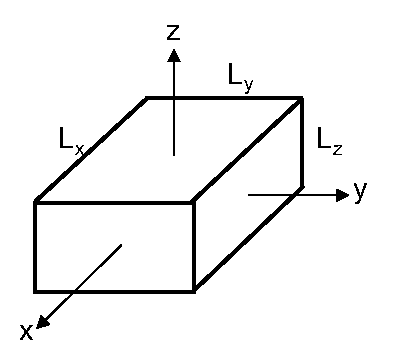
\includegraphics[width=1.3in]{Smatrix/Figures/Cuboid}}  & $L_xL_yL_z$ & $ \textrm{sinc}\left(\dfrac{L_x K_x}{2}\right)\textrm{sinc}\left(\dfrac{L_y K_y}{2}\right) \textrm{sinc}\left(\dfrac{L_z K_z}{2}\right)$  & $\textrm{sinc}(x) = \dfrac{\sin(x)}{x}$ \\   \hline

Circular Cylinder & \quad \parbox[c]{1em}{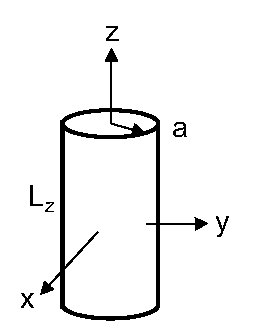
\includegraphics[width=0.9in]{Smatrix/Figures/Cylinder}}  & $\pi a^2 L_z$ & $ 2 \dfrac{ J_1(K_{\rho} a)}{ K_{\rho} a}  \textrm{sinc}\left(\dfrac{L_z K_z}{2}\right)$  & $K_{\rho} = \sqrt{K_x^2 + K_y^2} $ \\   \hline

Sphere & \parbox[c]{1em}{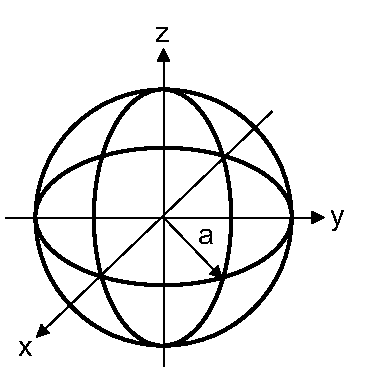
\includegraphics[width=1.2in]{Smatrix/Figures/Sphere}}  & $\dfrac{4}{3}\pi a^3$ & $ \dfrac{3(\sin(K a) - K a \cos(K a))}{(Ka)^3} $  & $K = \vert \bb{K} \vert $ \\   \hline

Ellipsoid & \parbox[c]{1em}{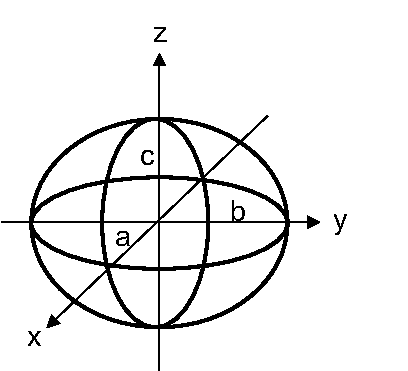
\includegraphics[width=1.3in]{Smatrix/Figures/Ellipsoid}}  & $\dfrac{4}{3}\pi abc$ & $ \dfrac{3(\sin(K') - K' \cos(K'))}{K'^3}   $  & $\begin{array}{c} K' = \vert \bb{K'} \vert \\ (K_x',K_y',K_z') = \\ (a K_x, b K_y, c K_z)\end{array}$ \\   \hline
\end{tabular}
\end{center}
\label{tablevolphaseint}
\end{table}%


\addtocontents{toc}{\protect\setcounter{tocdepth}{1}}
\subsection{Cuboid}
\addtocontents{toc}{\protect\setcounter{tocdepth}{2}}

Let a cuboid volume be centered at the origin with side lengths $L_x$, $L_y$, $L_z$ and let it be aligned with the Cartesian axes. In Cartesian coordinates, the volume phase integral, \eqref{volphaseint2}, becomes
\ea{
I &=& \int_{-L_x/2}^{L_x/2}  \int_{-L_y/2}^{L_y/2}  \int_{-L_z/2}^{L_z/2}  e^{i(K_x x + K_y y + K_z z)} dx dy dz }
%\ &=& \int_{-L_x/2}^{L_x/2} e^{i K_x x} dx  \int_{-L_y/2}^{L_y/2} e^{i K_y y} dy  \int_{-L_z/2}^{L_z/2}  e^{i K_z z} dz \\

The integral separates, then using the fact that 
\eq{\int_{-a/2}^{a/2} e^{i b z} dz = \dfrac{2}{b} \sin\left(\dfrac{ab}{2}\right) \label{sincinz}}

\noindent and multiplying top and bottom by $L_xL_yL_z$ to convert the sines to sinc functions the volume phase intergral over a cuboid is 
%\ea{I &=& \dfrac{4}{K_x K_y} \sin\left(\dfrac{L_x K_x}{2}\right)\sin\left(\dfrac{L_y K_y}{2}\right) \\
%\ & = & L_x L_y \textrm{sinc}\left(\dfrac{L_x K_x}{2}\right)\textrm{sinc}\left(\dfrac{L_y K_y}{2}\right) }

\eq{I  = L_x L_y L_z \textrm{sinc}\left(\dfrac{L_x K_x}{2}\right)\textrm{sinc}\left(\dfrac{L_y K_y}{2}\right) \textrm{sinc}\left(\dfrac{L_z K_z}{2}\right)}

\noindent where $\textrm{sinc} = \sin(x)/x$. This is equal to the volume of the cuboid times a product of directionally dependent $\textrm{sinc}$ functions.


\addtocontents{toc}{\protect\setcounter{tocdepth}{1}}
\subsection{Circular Cylinder}
\addtocontents{toc}{\protect\setcounter{tocdepth}{2}}

Let a circular cylinder be centered at the origin and aligned with the $z$ axis with radius $a$ and length $L_z$. The volume phase integral, \eqref{volphaseint2}, in cylindrical coordinates is written 
\ea{I  &=&  \int_{-L_z/2}^{L_z/2}  \int_0^{2\pi} \int_0^{a} e^{i (K_x \rho \cos\phi + K_y \rho \sin\phi + K_z z)} \rho d\rho d\phi dz }

\noindent where we have used the position vector $\br = \rho \cos\phi \hat{x} + \rho \sin\phi \hat{y} + \hat{z}$. The integral separates as 
\ea{I  &=& \int_0^{2\pi} \int_0^{a} e^{i (K_x \rho \cos\phi + K_y \rho \sin\phi)} \rho d\rho d\phi   \int_{-L_z/2}^{L_z/2} e^{i K_z z} dz }

The last integral is a sinc function in $z$ given by \eqref{sincinz}. Using the identity 
\eq{\int_0^{2\pi} e^{ u \cos t +v \sin t} d t = 2 \pi I_0 \left( \sqrt{u^2 + v^2} \right)}

\noindent the integral over $\phi$ evaluates to 
\eq{\int_0^{2\pi}  e^{i K_x \rho \cos\phi + K_y \rho \sin\phi} d\phi = 2\pi I_0 \left( i K_{\rho}  \rho \right)}

\noindent where $K_{\rho} = \sqrt{K_x^2 + K_y^2}$. The quantity $K_{\rho}$ is the component of the wave vector difference in the X-Y plane. Last, the integral in $\rho$ is evaluated using
\eq{\int_0^a I_0(i c x) x dx = \dfrac{a J_1(a c)}{c}}

Putting these together, the volume phase integral over a circular cylinder is
\ea{I  &=&   2\pi \dfrac{a J_1(K_{\rho} a)}{ K_{\rho} }  L_z \textrm{sinc}\left(\dfrac{L_z K_z}{2}\right)  }

Using the volume of the cylinder, $V = \pi a^2 L_z$, this can be written 
\ea{I  &=&  V   2 \dfrac{ J_1(K_{\rho} a)}{ K_{\rho} a}  \textrm{sinc}\left(\dfrac{L_z K_z}{2}\right)  }

Similar to the other shapes, this is equal to the volume of the cylinder multiplied by a directionally dependent term that has maximum value of 1.  


\addtocontents{toc}{\protect\setcounter{tocdepth}{1}}
\subsection{Sphere}
\addtocontents{toc}{\protect\setcounter{tocdepth}{2}}

\label{sectionvolintsphere}
Let a spherical volume with radius $a$ be centered at the origin. The volume phase integral, \eqref{volphaseint2}, can be written in spherical coordinates as 
\vspace{-2mm}
\eq{ I  =  \int_0^{2\pi} \int_0^{\pi} \int_0^a e^{i \bb{K} \cdot \br}  r^2 \sin\theta dr d\theta d\phi }

From symmetry, the dot product is evaluated relative to a common fixed axis such that $\bb{K} \cdot \br = K r \cos t$  where $t$ is the angle between $\bb{K}$ and $\br$. Using this, the integral becomes
\eq{ I  =  \int_0^{2\pi} \int_0^{\pi} \int_0^a e^{i K r \cos t}  r^2 \sin t dr dt d\phi \label{eqtemp21}}
\vspace{-2mm}

Next we use the identity 
\eq{j_n(z) = \dfrac{(-i)^n}{2} \int_0^{\pi} e^{i z \cos u} P_n(\cos u) \sin u du}

\noindent where $j_n(z)$ is the spherical Bessel function and $P_n(\cos u)$ is the Legendre polynomial. Applying this and integrating in $\phi$ \eqref{eqtemp21} becomes
\eq{ I  =  4\pi   \int_0^a j_0(K r) r^2 dr   \label{eqtmp22}}

Note that $j_0(x) = \sin(x)/x $.  This integral is given generally as
\eq{\int_0^a j_0 (c x) x^2 dx = \dfrac{\sin(a c) - a c \cos(a c)}{c^3}}

The volume phase integral over a sphere is given by
\eq{ I  =  4\pi \dfrac{\sin(K a) - K a \cos(K a)}{K^3}  \label{volphasphere1}   }

\noindent where $K$ is the magnitude of \eqref{Kvector}.  Using the volume of the sphere, $V = 4/3 \pi a^3$, this can be written
\ea{ I  &=&  V \dfrac{3(\sin(K a) - K a \cos(K a))}{(Ka)^3}}

%
%
%The volume phase integral over a sphere is given by
%\eq{ I  =  4\pi \dfrac{\sin(K a) - K a \cos(K a)}{K^3}  \label{volphasphere1}   }
%
%\noindent where $K$ is the magnitude of \eqref{Kvector}.  This can be written in terms of the volume of the sphere $V = 4/3 \pi a^3$ as 
%\ea{ I  &=&  V \dfrac{3(\sin(K a) - K a \cos(K a))}{(Ka)^3}}

The multiplying function acts like a directionally dependent weighting function that has a maximum value of 1 when $K a \rightarrow 0$.  

\addtocontents{toc}{\protect\setcounter{tocdepth}{1}}
\subsection{Ellipsoid}
\addtocontents{toc}{\protect\setcounter{tocdepth}{2}}

Let an ellipsoid be centered on the origin with axes $(a, b, c)$ along XYZ, respectively. We define a new position vector, $\br'$, in spherical coordinates using the change of variables 
\ea{\br' &=& r a \sin\theta\cos\phi \hat{x} + r b \sin\theta\sin\phi \hat{y} +  r c\cos\theta \hat{z} \\
dV &=& abc r^2 \sin\theta dr d\theta d\phi}

The volume phase integral, \eqref{volphaseint2}, can then be written as an integral over the unit sphere
\eq{ I  =  abc \int_0^{2\pi} \int_0^{\pi} \int_0^1 e^{i \bb{K} \cdot \br'}  r^2 \sin\theta dr d\theta d\phi }

Next, transfer the coefficients $(a,b,c)$ that are in $\br'$ to a new wave vector difference, $\bb{K}'$, so that, $(K_x',K_y',K_z') = (a K_x, b K_y, c K_z)$. The position vector returns to its unstretched form and we have
\eq{ I  =  abc \int_0^{2\pi} \int_0^{\pi} \int_0^1 e^{i \bb{K}' \cdot \br}  r^2 \sin\theta dr d\theta d\phi }

Using the results of Section \ref{sectionvolintsphere}, \eqref{volphasphere1}, the volume phase integral over an ellipsoid is 
\eq{ I  =  4\pi abc \dfrac{\sin(K') - K' \cos(K')}{K'^3}     }

\noindent where $K'$ is the magnitude of $\bb{K}'$.  The volume of an ellipsoid is $V = 4/3\pi abc$, and this can be written
\eq{ I  =  V \dfrac{3(\sin(K') - K' \cos(K'))}{K'^3}     }

\clearpage



\clearpage
\newpage










